 \documentclass{article}
\usepackage{graphicx} % Required for inserting images
\usepackage[left=2.5cm, right=2.5cm, top=2cm, bottom=2cm]{geometry}
\usepackage{xcolor}
\usepackage{hyperref}
\usepackage{float}
\usepackage{url}


\title{CSE474/574 Introduction to Machine Learning \\ \vspace{0.5cm} \large Course Syllabus}
\author{}
\date{}
\begin{document}

\maketitle

\section{Introduction}
Involves teaching computer programs to improve their performance through guided training and unguided experience. Takes both symbolic and numerical approaches. Topics include concept learning, decision trees, neural nets, latent variable models, probabilistic inference, time series models, Bayesian learning, sampling methods, computational learning theory, support vector machines, and reinforcement learning.

This course will equip students with the necessary skills to become a machine learning engineer. In addition to the machine learning algorithms, we will discuss how to handle large datasets and the latest approach to handling streaming datasets.
\subsection{Instructor Information}
\begin{itemize}
    \item \textbf{Instructor}: Jue Guo
    \item \textbf{Office Hr}: Monday 9:00AM -- 10:30AM
    \item \textbf{Location}: \href{https://buffalo.zoom.us/j/7673733717?pwd=TktTVXlDOGgxM3dRUC9UT21hNEdOQT09&omn=92002344719}{Zoom Link}
    \item Read piazza post frequently.
\end{itemize}
\subsection{Course Location and Time}
\begin{itemize}
    \item \textbf{Location}: Norton 190
    \item \textbf{Time}: Monday, Wednesday, and Friday, 3:00 pm to 3:50 pm.
    \item Drop Date: 1/31/24
    \item Attendance is not mandatory, and all the course note will be handwritten in class. Course material on GitHub can be used as a guide but not the ultimate contents being conveyed in class.
\end{itemize}

\subsection{Course Material}
You \textbf{do not} need to buy or download pdf of these books;
\begin{itemize}
    \item \textit{\textbf{Pattern Classification}, David G. Stork, Peter E. Hart, and Richard O. Duda}
    \item \textit{\textbf{Pattern Recognition and Machine Learning}, Christopher Bishop}
    \item  \textit{\textbf{Deep Learning}, Goodfellow Ian, Yoshua Bengio, and Aaron Courville}
\end{itemize}

\subsection{What is Machine Learning?}
\begin{figure}[H]
    \centering
    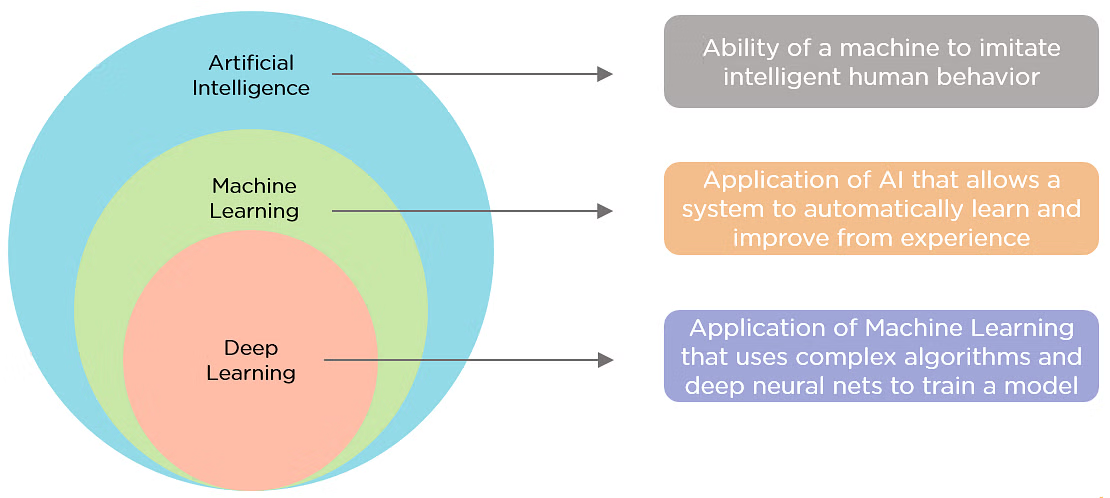
\includegraphics[scale=0.3]{image.png}
    \caption{Relationship between Machine Learning, Artificial Intelligence and Deep Learning}
\end{figure}
\section{Course Outline}
The course will be split into five parts\footnote{The instructor has the right to change the content of the course as the instructor sees fit}. Remember it is a STEM class, so expect math and engineering:

\begin{table}[htbp]
    \centering
    \begin{tabular}{|c|c|}
        \hline
        \textbf{Weeks} & \textbf{Course Material}                                      \\
        \hline
        1,2,3          & Introduction \& Notation \& Basic Algorithms                  \\
        \hline
        5,6            & Anatomy of Learning Algorithms \& Basic Practice              \\
        \hline
        7              & Mid-Term                                                      \\
        \hline
        8,9            & Neural Networks \& Advance Practices \& Unsupervised Learning \\
        \hline
        9,10           & Robustness: Adversarial attack \& training                    \\
        \hline
        11,12          & Deal with Continuous Data: Continual Learning                 \\
        \hline
        13             & Final                                                         \\
        \hline
    \end{tabular}
    \caption{Course Outline}
\end{table}
This is a 15 week course; I left two weeks out in the outline above just in case we need it.
\begin{figure}[H]
    \centering
    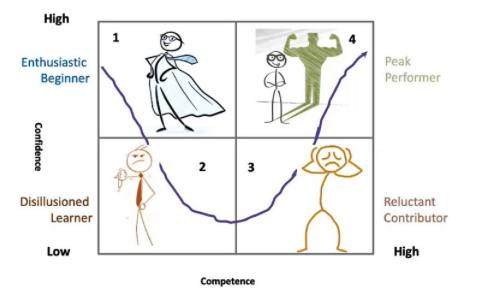
\includegraphics[width=0.6\linewidth]{lr_curve.png}
\end{figure}
\section{Evaluation}
The course will have \textbf{three} programming assignments(PA), \textbf{weekly} quiz every Friday, \textbf{one} midterm, and \textbf{one} final.

\begin{table}[htbp]
    \centering
    \begin{tabular}{|c|c|}
        \hline
        \textbf{Requirement}               & \textbf{Weight} \\
        \hline
        PA1: Supervised Algorithms         & 10 \%           \\
        \hline
        PA2: Unsupervised Algorithms       & 10 \%           \\
        \hline
        PA3: CNNs and Adversarial Training & 15 \%           \\
        \hline
        Weekly Quiz                        & 15 \%           \\
        \hline
        Mid-Term                           & 25 \%           \\
        \hline
        Final                              & 25 \%           \\
        \hline
    \end{tabular}
    \caption{Evaluation Distribution}
\end{table}
After we release the grade, you will have exactly \textbf{one week} to ask the TA or Grader for re-evaluation.  We will not indulge in your regrade request after re-evaluation period. During the evaluation, your grade may go down if we found additional problems. No \textbf{bonus} is provided, if you want an A, you have to earn it.

\subsection{Grade}
This course is \textbf{absolute} grading, meaning no curve, as there is a certain standard we need to uphold for students to have a good knowledge of machine learning.
\begin{table}[htbp]
    \centering
    \begin{tabular}{|c|c|c|c|}\hline \textbf{Percentage} & \textbf{Letter grade} & \textbf{Percentage} & \textbf{Letter grade} \\ \hline \(95-100\) & \(\mathrm{~A}\) & \(70-74\) & \(\mathrm{C}+\) \\ \hline \(90-94\) & \(\mathrm{~A}-\) & \(65-69\) & \(\mathrm{C}\) \\ \hline \(85-89\) & \(\mathrm{~B}+\) & \(60-64\) & \(\mathrm{C}-\) \\ \hline \(80-84\) & \(\mathrm{~B}\) & \(55-59\) & \(\mathrm{D}\) \\ \hline \(75-79\) & \(\mathrm{~B}-\) & \(0-54\) & \(\mathrm{~F}\) \\ \hline\end{tabular}
\end{table}
If the course is undergraduate and graduate level combined. The \textbf{undergraduate section} will have a 5 percent bonus for this course and it is automatically included in the final grade.
\section{Incomplete (I) grades}
A grade of incomplete (“I”) indicates that additional coursework is required to fulfill the requirements of a given course. Students may only be given an “I” grade if they have a passing average in coursework that has been completed and have well-defined parameters to complete the course requirements that could result in a grade better than the default grade. An “I” grade may not be assigned to a student who did not attend the course.

Prior to the end of the semester, students must initiate the request for an “I” grade and receive the instructor’s approval. Assignment of an “I” grade is at the discretion of the instructor.

The last day to resign the course is Thursday, March 2, 2023.

\section{Academic Integrity}
Academic integrity is a fundamental university value. Through the honest completion of academic work, students sustain the integrity of the university while facilitating the university's imperative for the transmission of knowledge and culture based upon the generation of new and innovative ideas. Please refer to the university Undergraduate Academic Integrity Policy (\url{https://catalog.buffalo.edu/policies/academic_integrity_2019-20.html}) for additional information.

As an engineer or computer scientist, you have special ethical obligations. As per the NSPE Code of Ethics, “engineers shall avoid deceptive acts” and “shall conduct themselves honorably, responsibly, ethically, and lawfully so as to enhance the honor, reputation, and usefulness of the profession (\url{https://www.nspe.org/resources/ethics/code-ethics}). Similar sentiments of honesty, integrity, fairness, and responsibility are fundamental to the ACM Code of Ethics (\url{https://www.acm.org/code-of-ethics}).

A violation in this class generally results in an F for the entire course. The Computer Science and Engineering department's policy on academic integrity can be found here:
\href{https://engineering.buffalo.edu/computer-science-engineering/information-for-students/undergraduate-program/cse-undergraduate-academic-policies/cse-academic-integrity-policy.html}{CSE Academic Integrity Policy}



\section{What Constitutes a Violation of Academic Integrity?}
These bullets should be obvious things not to do (but commonly occur):
\begin{itemize}
    \item Turning in your friend’s code/write-up (obvious).
    \item Turning in solutions you found on Google with all the variable names changed (should be obvious). This is a copyright violation, in addition to an AI violation.
    \item Turning in solutions you found on Google with all the variable names changed and 2 lines added (should be obvious). This is also a copyright violation.
    \item Paying someone to do your work. You may as well not submit the work since you will fail the exams and the course.
    \item Posting to forums asking someone to solve the problem. Note: Aggregating every [ stack overflow answer $\mid$ result from google $\mid$ other source ] because you "understand it" will likely result in full credit on assignments (if you aren't caught) and then failure on every exam. \textbf{Exams don't test if you know how to use Google, but rather test your understanding (i.e., can you understand the problems to arrive at a solution on your own).} Also, other students are likely doing the same thing and then you will be wondering why 10 people that you don’t know have your solution.
\end{itemize}
Other violations that may not be as obvious:
\begin{itemize}
    \item Working with a tutor who solves the assignment with you. If you have a tutor, please contact me so that I may discuss with them what help is allowed.
    \item Sending your code to a friend to help them. If another student uses/submits your code, you are also liable and will be punished.
    \item Joining a chatroom for the course where someone posts their code once they finish, with the honor code that everyone needs to change it in order to use it.
    \item Reading your friend’s code the night before it is due because you just need one more line to get everything working. It will most likely influence you directly or subconsciously to solve the problem identically, and \textbf{your friend will also end up in trouble}.
\end{itemize}

\section{What Collaboration is Allowed?}
Assignments in this course should be solved individually with only assistance from course staff and allowed resources. You may discuss and help one another with technical issues, such as how to get your compiler running, etc.

There is a gray area when it comes to discussing the problems with your peers, and I do encourage you to work with one another to solve problems. That is the best way to learn and overcome obstacles. At the same time, you need to be sure you do not overstep and not plagiarize. Talking out how you eventually reached the solution from a high level is okay: "I used a stack to store the data and then looked for the value to return." but explaining every step in detail/pseudocode is not okay: "I copied the file tutorial into my code at the start of the function, then created a stack and pushed all of the data onto the stack, and finished by popping the elements until the value is found and use a return statement." The first example is OK but the second is basically a summary of your code and is not acceptable, and remember that you shouldn’t be showing any code at all for how to do any of it. Regardless of where you are working, you must always follow this rule: Never come away from discussions with your peers with any written work, either typed or photographed, and especially do not share or allow viewing of your written code.

\section{Resources are Allowed?}
With all of this said, please feel free to use any [files|examples|tutorials] that we provide directly in your code (with proper attribution). Feel free to directly use anything from lectures or recitations. You will never be penalized for doing so, but should always provide attribution/citation for where you retrieved code from. Just remember, if you are citing an algorithm that is not provided by us, then you are probably overstepping.

More explicitly, you may use any of the following resources (with proper citation/attribution in your code):
\begin{itemize}
    \item Any example files posted on the course webpage (from lecture or recitation).
    \item Any code that the instructor provides.
    \item Any code that the TAs provide.
\end{itemize}
Omitting citation/attribution will result in an AI violation (and lawsuits later in life at your job). This is true even if you are using resources provided.

\section{Amnesty Policy}
We understand that students are under a lot of pressure and people make mistakes. If you have concerns that you may have violated academic integrity on a particular assignment, and would like to withdraw the assignment, you may do so by sending me an email \textbf{BEFORE THE VIOLATION IS DISCOVERED BY ME}. The email should take the following format:
\begin{quote}
    Dear Professor/TAs,

    I wish to inform you that on assignment X, the work I submitted was not entirely my own. I would like to withdraw my submission from consideration to preserve academic integrity.

    Sincerely, J

    Student Person \# 12345678 UBIT: jqstuden
\end{quote}
When we receive this email, student J would receive a 0 on assignment X, but would not receive an F for the course, and would \textbf{not} be reported to the office of academic integrity.

\section{Critical Campus Resources}
\subsection{Accessibility Resources}
If you have any disability which requires reasonable accommodations to enable you to participate in this course, please contact the Office of Accessibility Resources in 60 Capen Hall, 716-645-2608 and also the instructor of this course during the first week of class. The office will provide you with information and review appropriate arrangements for reasonable accommodations, which can be found on the web at:\url{http://www.buffalo.edu/studentlife/who-we-are/departments/accessibility.html}.

\subsection{Sexual Violence}
UB is committed to providing a safe learning environment free of all forms of discrimination and sexual harassment, including sexual assault, domestic and dating violence and stalking. If you have experienced gender-based violence (intimate partner violence, attempted or completed sexual assault, harassment, coercion, stalking, etc.), UB has resources to help. This includes academic accommodations, health and counseling services, housing accommodations, helping with legal protective orders, and assistance with reporting the incident to police or other UB officials if you so choose. Please contact UB’s Title IX Coordinator at 716-645-2266 for more information. For confidential assistance, you may also contact a Crisis Services Campus Advocate at 716-796-4399.

\subsection{Mental Health}
As a student, you may experience a range of issues that can cause barriers to learning or reduce your ability to participate in daily activities. These might include strained relationships, anxiety, high levels of stress, alcohol/drug problems, feeling down, health concerns, or unwanted sexual experiences. Counseling, Health Services, and Health Promotion are here to help with these or other issues you may experience. You can learn more about these programs and services by contacting:
\begin{itemize}
    \item Counseling Services:
          \begin{itemize}
              \item 120 Richmond Quad (North Campus), 716-645-2720
              \item 202 Michael Hall (South Campus), 716-829-5800
          \end{itemize}
    \item Health Services:
          \begin{itemize}
              \item 4350 Maple Rd, Amherst, NY 14226, 716-829-3316
          \end{itemize}
    \item Health Promotion:
          \begin{itemize}
              \item 114 Student Union (North Campus), 716-645-2837
          \end{itemize}
\end{itemize}

\subsection{Diversity}
The UB School of Engineering and Applied Sciences considers the diversity of its students, faculty, and staff to be a strength, critical to our success. We are committed to providing a safe space and a culture of mutual respect and inclusiveness for all. We believe a community of faculty, students, and staff who bring diverse life experiences and perspectives leads to a superior working environment, and we welcome differences in race, ethnicity, gender, age, religion, language, intellectual and physical ability, sexual orientation, gender identity, socioeconomic status, and veteran status.


\end{document}